\documentclass[runningheaders,a4paper]{llncs}

\usepackage[ngerman]{babel}
\usepackage{graphicx}
\usepackage[utf8]{inputenc}
\usepackage[T1]{fontenc}
% Darstellung von URLs
\usepackage{url}
\usepackage{amsmath,amssymb}
\usepackage{listings}
\usepackage{subfig}
\usepackage{multirow}
\usepackage{array}
\usepackage{svg}
\usepackage{listings}
\lstset{language=C++}

\usepackage{tikz}
\usetikzlibrary{calc, arrows,shapes,snakes,automata,backgrounds,petri}
\tikzset{
	%Define standard arrow tip
	>=stealth',
	%Define style for different line styles
	help lines/.style={dashed, thick},
	axis/.style={<->},
	line/.style={thick};
}

\usepackage[]{algorithm2e}
\pagestyle{plain}

%für pseudocode:
\SetKwProg{Fn}{Function}{}{end}\SetKwFunction{FRecurs}{FnRecursive}%
\SetAlgoLongEnd

% Benötigte Angaben für die Titelseite
\title{ Moment Shadow Mapping, Moment Based Volumetric Obscurance und Sample Distribution Shadow Maps }

\author{
	Akasha Jethwa 
	Matrikel-Nr: 2563201
	\and
	Jonas Weinz 
	Matrikel-Nr: 2571421
	\and
	Tom Kneiphof 
	Matrikel-Nr: 2662506
}

% Hier das Institut angeben
\institute{Institut für Informatik der Universität Bonn}

\begin{document}

% Erstellung des Titels
\maketitle

\begin{abstract}
Dieser Bericht ist Teil einer Projektgruppe am Institut für Informatik der Universität Bonn,
die sich mit der Implementierung drei verschiedener Echtzeit-Renderingtechniken für Schatten beschäftigt.
In diesem Bericht wird die Funktionsweise und Implementierung von Sample Distribution Shadow Maps, Volumetric-Obscurance und Moment Shadow Mapping behandelt.
Alle drei Techniken werden in einer kleinen Engine implementiert und in einem Demo-Spiel verwendet.
\end{abstract}


\section{Einleitung}
Rendern von Schatten ist ein wichtiger Aspekt der interaktiven 3D Grafik.
Die Struktur einer Szene wirkt erst durch Schatten realisitisch und hilft dem Betrachter dabei, Relationen zwischen Objekten besser zu verstehen.
Allerdings ist das Berechnen der verschiedenen Schattentechniken aufwendig und oft anfällig für Fehlerartefakte.
Deshalb untersuchen wir in diesem Paper 3 Techniken, welche verschiedene Lösungsansätze und Vorteile bieten.
Zusätzlich implementieren wir alles in einer eigenen 3D Engine und generieren daraus ein kurzes Spiel um die Techniken zu demonstrieren.


% Introduction
\subsection{Sample Distribution Shadow Maps}

Ein häufiges Problem bei der Shadow Map Generierung ist Aliasing durch Over und Under Sampling.
Sample Distribution Shadow Maps (SDSMs) \cite{sdsm} sind ein voll automatisches Verfahren mit konstantem Speicherbedarf und einer vorhersagbaren Worst-Case Laufzeit, die nicht von der Szenenkomplexität abhängt.
Das Verfahren ist dadurch sehr gut für den Einsatz in Echtzeit Grafikanwendungen geeignet.
SDSM ist ein Screen Space Verfahren, welches adaptiv in jedem Frame Z-Partitionen \cite{zpart} (Hier auch Kaskaden \cite{csm}) erstellt.
So wird mehr Shadow Map Auflösung für Bereiche in der nähe der Kamera zur Verfügung gestellt und weniger für weit entfernte Bereiche, wodurch Perspektivischem Aliasing entgegen gewirkt wird.
Des Weiteren werden die Shadow Map Frusta von SDSMs eng um die tatsächlich sichtbare Geometrie gelegt, was die zur verfügung Stehende Auflösung in den Shadow Maps zusätzlich erhöht.


% Introduction
\subsection{Volumetric Obscurance}
Obscurance (= Umgebungsverdeckung) ist eine Technik zur Berechnung von Schatten basierend auf der Annahme,
dass sich gegenseiteg verdeckende Geometrie zu einem verringertem Lichteinfall führt. In diesem Paper werden
wir verschiedene Screenspace Algorithmen für Volumetric Obscurance erläutern und kurz unsere Implementationen vorstellen.


% Introduction
\subsection{Moment Shadow Mapping}
Wir wollen eine Schattentechnik verwenden, die möglichst hohe Qualität liefert und dabei performant bleibt. Wünschenswert, wäre ebenfalls filterbare Shadow Maps und eine performante Methode. Moment Shadow Mapping liefert uns dieses Verfahren und wird im weiteren Verlauf erläutert und implementiert.



\section{Related Work}

% Related Work
\subsection{Sample Distribution Shadow Maps}

Parallel Split Shadow Maps (PSSMs) \cite{pssm} ist ein existierendes Verfahren um Perspektivisches Aliasing zu minimieren.
Allerdings liefert es nicht immer gute Ergebnisse und hängt von Parametern ab, deren optimaler Wert unbekannt ist.

Andere Verfahren wie Adaptive Shadow Maps \cite{asm} und Resolution-Matched Shadow Maps \cite{rmsm} verwalten eine komplexe Baumstruktur von Shadow Maps um die Shadow Map Auflösung adaptiv in der Szene zu verteilen.
Sie erreichen eine hohe Qualität auf Kosten von Performanz, wodurch sie für Echtzeitanwendungen eher ungeeignet sind.


% Related Work
\subsection{Volumetric Obscurance}

Ambient Occlusion (= Umgebungsverdeckung) ist eine weit verbreitete Technik um Schatten in 3D-Szenen
zu approximieren. Dafür gibt es allgemein 2 Ansätze:
\begin{enumerate}
	\item "Global Ambient Occlusion": für jeden Punkt in der Szene wird geprüft, ob der Himmel von diesem
		Punkt aus sichtbar ist (bzw. bei geschlossenen Szenen: ob eine maximale Distanz ohne Kollision erreicht
		 werden kann). Dieses Verfahren ist relativ teuer, kann aber z.B. für statische Szenen vorberechnet
		 werden.
		\cite{aoPaper}
	\item Screenspace Ambient Occlusion (SSAO): für jeden Pixel im Screenspace werden Point Samples
		innerhalb einer bestimmten Umgebung erstellt. Mit Hilfe der Tiefeninformationen des Depth Buffers
		wird die Anzahl der Samples, die hinter der Szenengeometrie liegen müssen bestimmt. Anhand dieser Anzahl
		kann der Pixel entsprechend abgedunkelt werden.  \cite{cry2Paper}
\end{enumerate}  
Volumetric Obscurance ist eine Alternative zum Screenspace Volumetric Obscurance, welche wir im folgenden
Erläutern werden

\cite{loos2010volumetric}

% Related Work
\subsection{Moment Shadow Mapping}

Moment Shadow Mapping \cite{msm}, Variance Shadow Maps \cite{donnelly2006variance}, Percentage Closer Filtering \cite{reeves1987rendering}

Im Gegensatz zu normalen Texturen, können Shadow Maps nicht einfach gefiltert werden um Aliasing zu verhindern. Percentage Closer Filtering ist ein Ansatz um dies zu ermöglichen und Aliasing zu vermindern. Diese Technik versucht den Prozentwert eines Objekts zu erkennen, welcher näher an der Lichtquelle liegt und nicht im Schatten. Mithilfe von Chebichev's Ungleichung, lässt sich so eine exaktere approximierung für PCF erreichen \cite{vsm}

Variance Shadow Maps benutzt 2 Momente und löst das General Moment Problem. Ein filtern ist  möglich und PCF wird weiter verbessert bzw. approximiert. VSM ist hinsichtlich der MSM ein spezialfall für $m = 2$, also 2 statt 4 Momenten. Normalerweise betrachten wir die Tiefe um eine Shadow Map zu Rendern. VSM nutzt die Tiefe und die quadrierte Tiefe und speichert diese in einem 2-Kanal Buffer. Der Vorteil liegt dara, dass nu Pre-Processing Effekte genutzt werden um die so erstellte Variance Shado Map zu filtern.\cite{donnelly2006variance}

Desweiteren betrachen wir Moment Based Volumetric Obscurance. Die eigentliche Volumetric Obscurance wird in den entsprechen Abschnitten weiter erläutert.

% Main
\section{Sample Distribution Shadow Maps}

Sample Distribution Shadow Maps (SDSMs) ist ein Verfahren zur adaptiven Optimierung der Shadow Map Auflösung unter Verwendung des Camera-Space Depth Buffers.

% SDSM
\subsection{Algorithmus}

% Cascaded Shadow Maps aka Z-Partitioning
SDSMs basieren auf Z-Partitoning, wobei das Kamera Frustum entlang der Blickrichtung in mehrere Kaskaden partitioniert wird. Für jedes Kaskade wird eine eigene Shadow Map generiert.
Auf diese Weise kann mehr Shadow Map Auflösung für nahe Objekte verwendet werden, und weniger Auflösung für weit entfernte Objekte.


% Betrachte Punkte in Light-Space TODO
Der Algorithmus betrachtet die Verteilung aller sichtbaren Punkte der Szene aus der Sicht des Lichtes (im Light Space).
Hierzu wird für jedes Sample aus dem Camera Depth Buffer die Position in der Welt rekonstruiert und in den Light Space transformiert.
Die so erhaltenen Punkte sind genau die, für die beim Rendern der Szene aus der Sicht der Kamera auf die Shadow Map zugegriffen wird.


% Partitionierung
Für gute Ergebnisse ist eine geeignete Wahl der Partition ausschlaggebend.
Anstatt auf eine statische Partitionierung des Kamera Frustums \cite{pssm} zu setzen, wird die Partitionierung von SDSMs in jedem Frame neu berechnet, so dass sie die sichtbare Geometrie optimal abdeckt.

% - Min/Max Reduktion
% - Logarithmische Partitionierung
Zunächst wird die tatsächliche Near und Far Distanz der sichtbaren Geometrie im Kamera Frustums ermittelt.
Dies geschieht mittels Min/Max Reduktion der Tiefenwerte im Kamera Depth Buffer.
Anschließend wird das Kamera Frustum zwischen tatsächlicher Near und Far Distanz logarithmisch partitioniert um das perspektivische Aliasing zu minimieren.

% Abgrenzung PSSM Logarithmic/Linear
PSSMs kennen die tatsächliche Near und Far Distanz nicht, und müssen mit der Near und Far Distanz der Projektionsmatrix arbeiten.
Eine logarithmische Partitionierung würde zu viel Shadow Map Auflösung in den sehr nahen Bereich verschieben, der oft leer ist.
PSSMs konvexkombinieren die Partitionsgrenzen der linearen und logarithmischen Partitionierung um mehr Auflösung von der Near Plane weg zu bewegen.
Optimale Koeffizienten müssen meist von Hand ermittelt werden.

% (K-Means and friends)
Weitere Möglichkeiten das Kamera Frustum intelligent zu partitionieren, sind ein adaptiv logarithmisches und ein K-Means Verfahren.
Das adaptiv logarithmische Verfahren vermeidet Lücken im Histogramm des Kamera Depth Buffers, indem es die Partitionsgrenzen an das Ende von diesen schiebt.
Das K-Means Verfahren sucht zunächst Maxima im Histogramm des Kamera Depth Buffers und legt dann die Partition entsprechend um die gefundenen Maxima.
Für beide Verfahren muss zunächst das Histogramm des Camera Depth Buffers berechnet werden.


% Tight Partition Frusta
Andere Algorithmen wie PSSM \cite{pssm} projizieren die Ecken des Kamera Frustums bzw. der Kaskaden in den Light Space um das Frustum für die Shadow Map zu erhalten.
Um das Frustum möglichst klein zu wählen kann dort eine Oriented Bounding Box anstelle einer Axis Aligned Bounding Box (AABB) berechnet werden.
Die Konvexe Hülle der in den Light Space projizierten Punkte kann ein sehr komplexes Polygon werden, weshalb es sich für SDSMs nicht lohnt diese zu berechnen.

SDSMs berechnen für jede Kaskade eine AABB, die dann das Frustum für die Shadow Map bildet.
Damit die AABBs die sichtbare Geometrie sinnvoll umschließen, wird der Light Space so rotiert, dass die Z-Achse des Camera Spaces sich an der X-Achse des Light Spaces ausgerichtet


% SDSM Cascades colorized
\begin{figure}
	\centering
	\subfloat{
		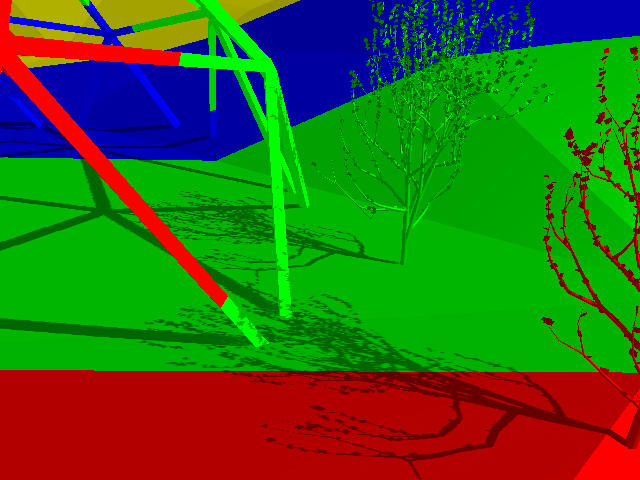
\includegraphics[width=5.5cm]{sdsm_assets/pssm_colorized_near.png}
	}
	\subfloat{
		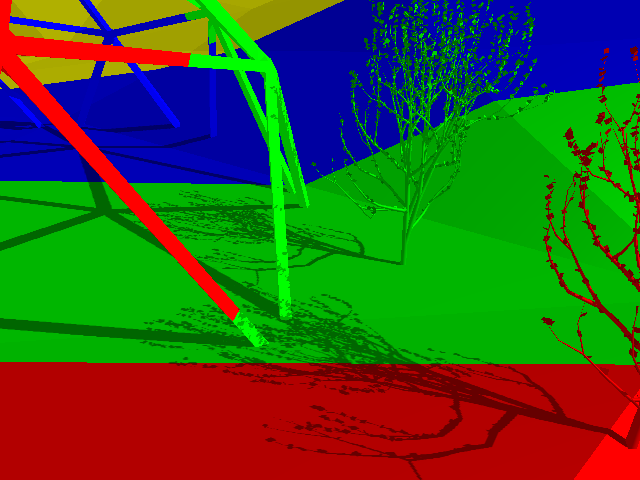
\includegraphics[width=5.5cm]{sdsm_assets/sdsm_colorized_near.png}
	}

	\subfloat{
		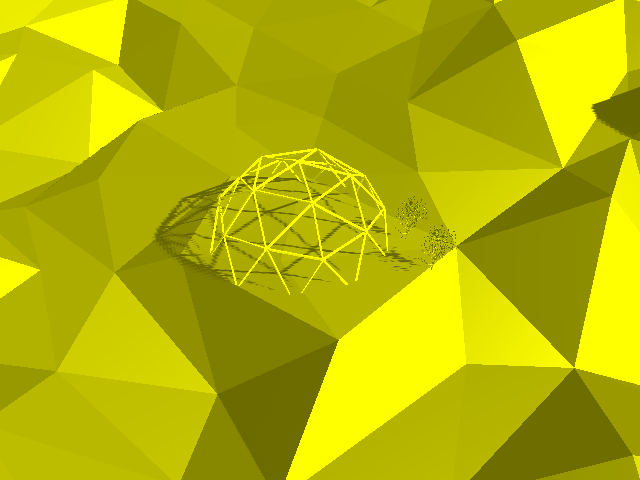
\includegraphics[width=5.5cm]{sdsm_assets/pssm_colorized_far.png}
	}
	\subfloat{
		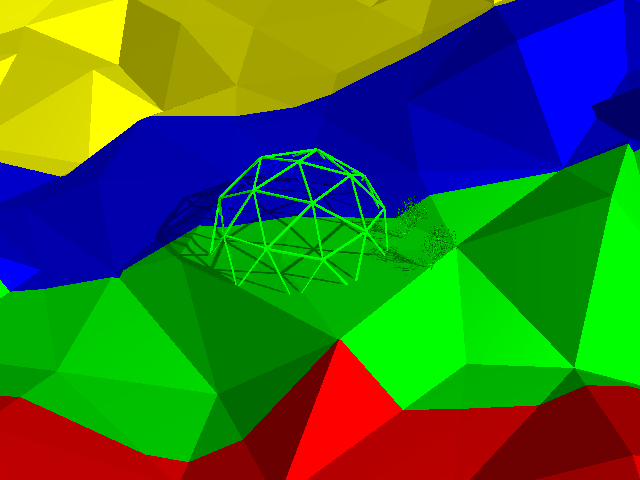
\includegraphics[width=5.5cm]{sdsm_assets/sdsm_colorized_far.png}
	}

	\caption{
Visualisierung der Kaskaden in den Farben rot (nah), grün, blau, gelb (fern).
Links sind Partitionierungen durch Parallel Split Shadow Maps zu sehen.
Rechts sind Partitionierungen durch Sample Distribution Shadow Maps zu sehen.
Die Partitionierung der PSSMs ist für das obere linke Bild optimiert.
Während SDSMs die Kaskaden unten rechts adaptiv anpassen können, versagen die PSSMs in dem unteren linken Bild.
}
\end{figure}


% SDSM Camera View
\begin{figure}
	\centering
	\subfloat[PSSM] {
		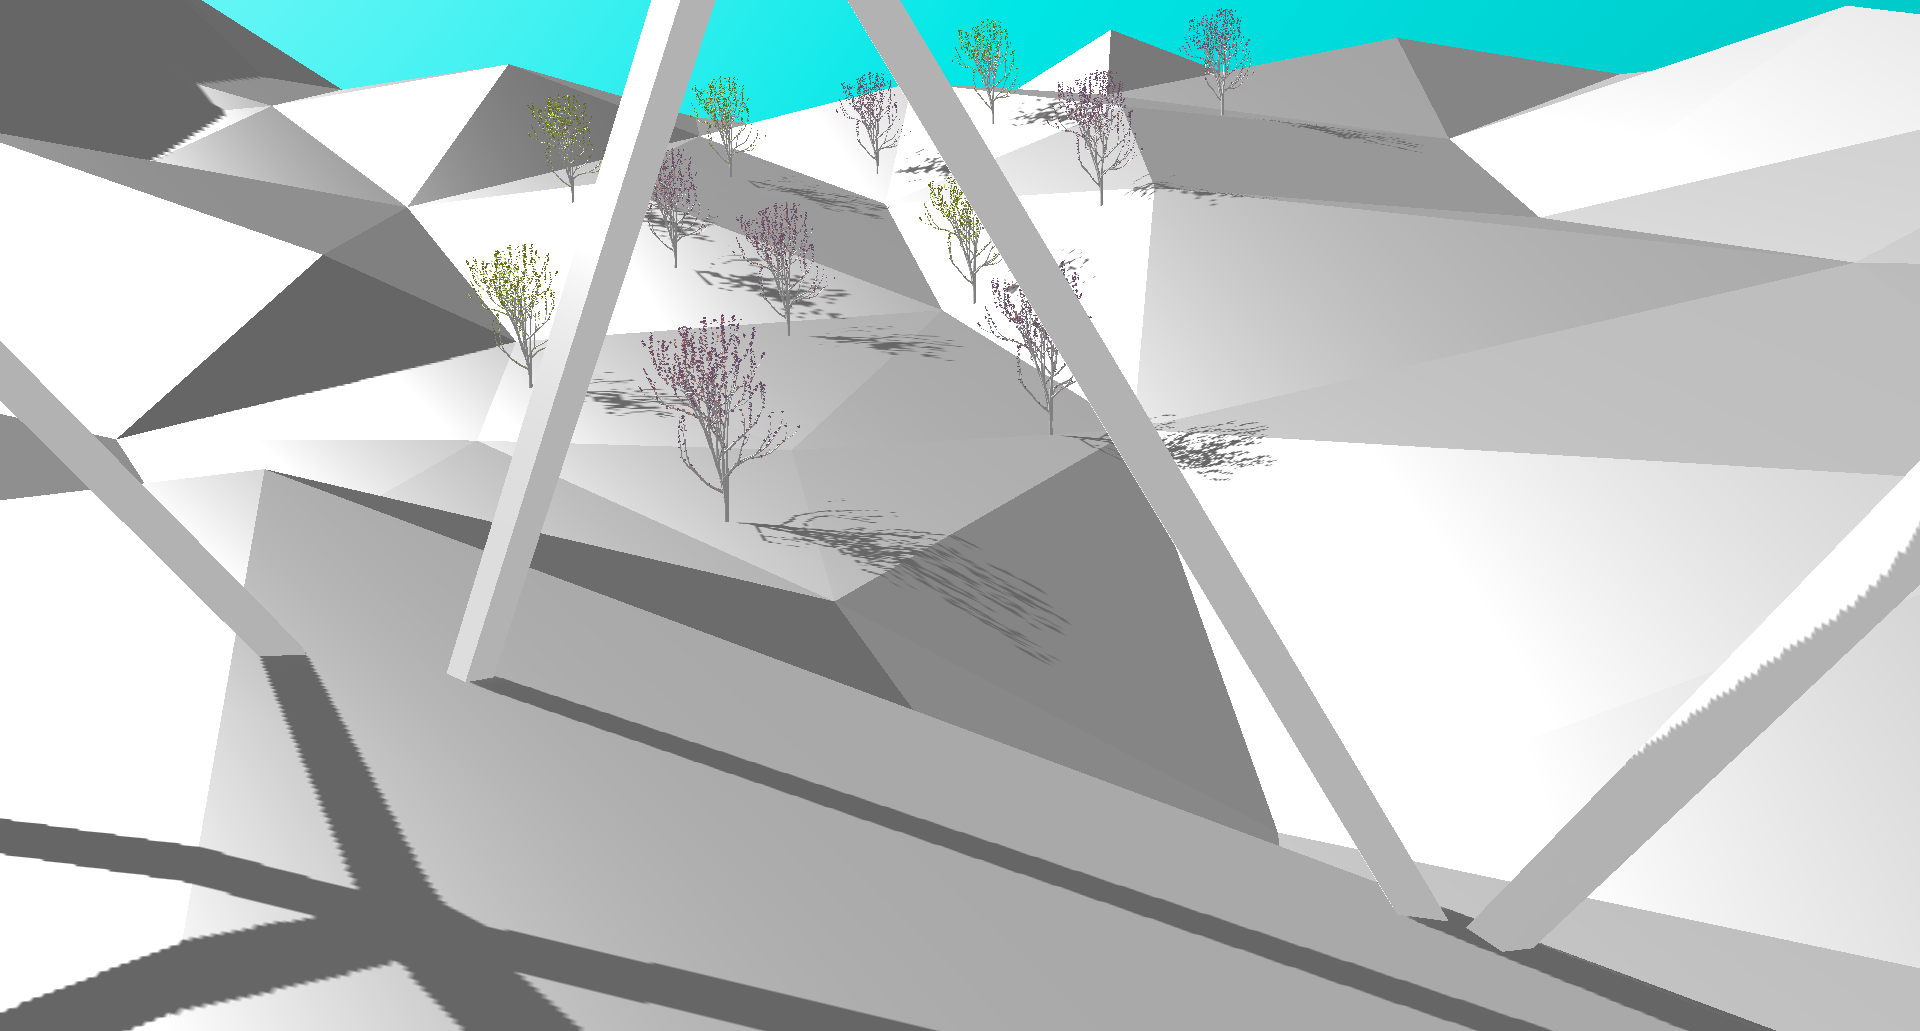
\includegraphics[width=5.5cm]{sdsm_assets/pssm_scene.png}
		\label{ref:pssm_scene}
	}
	\subfloat[SDSM] {
		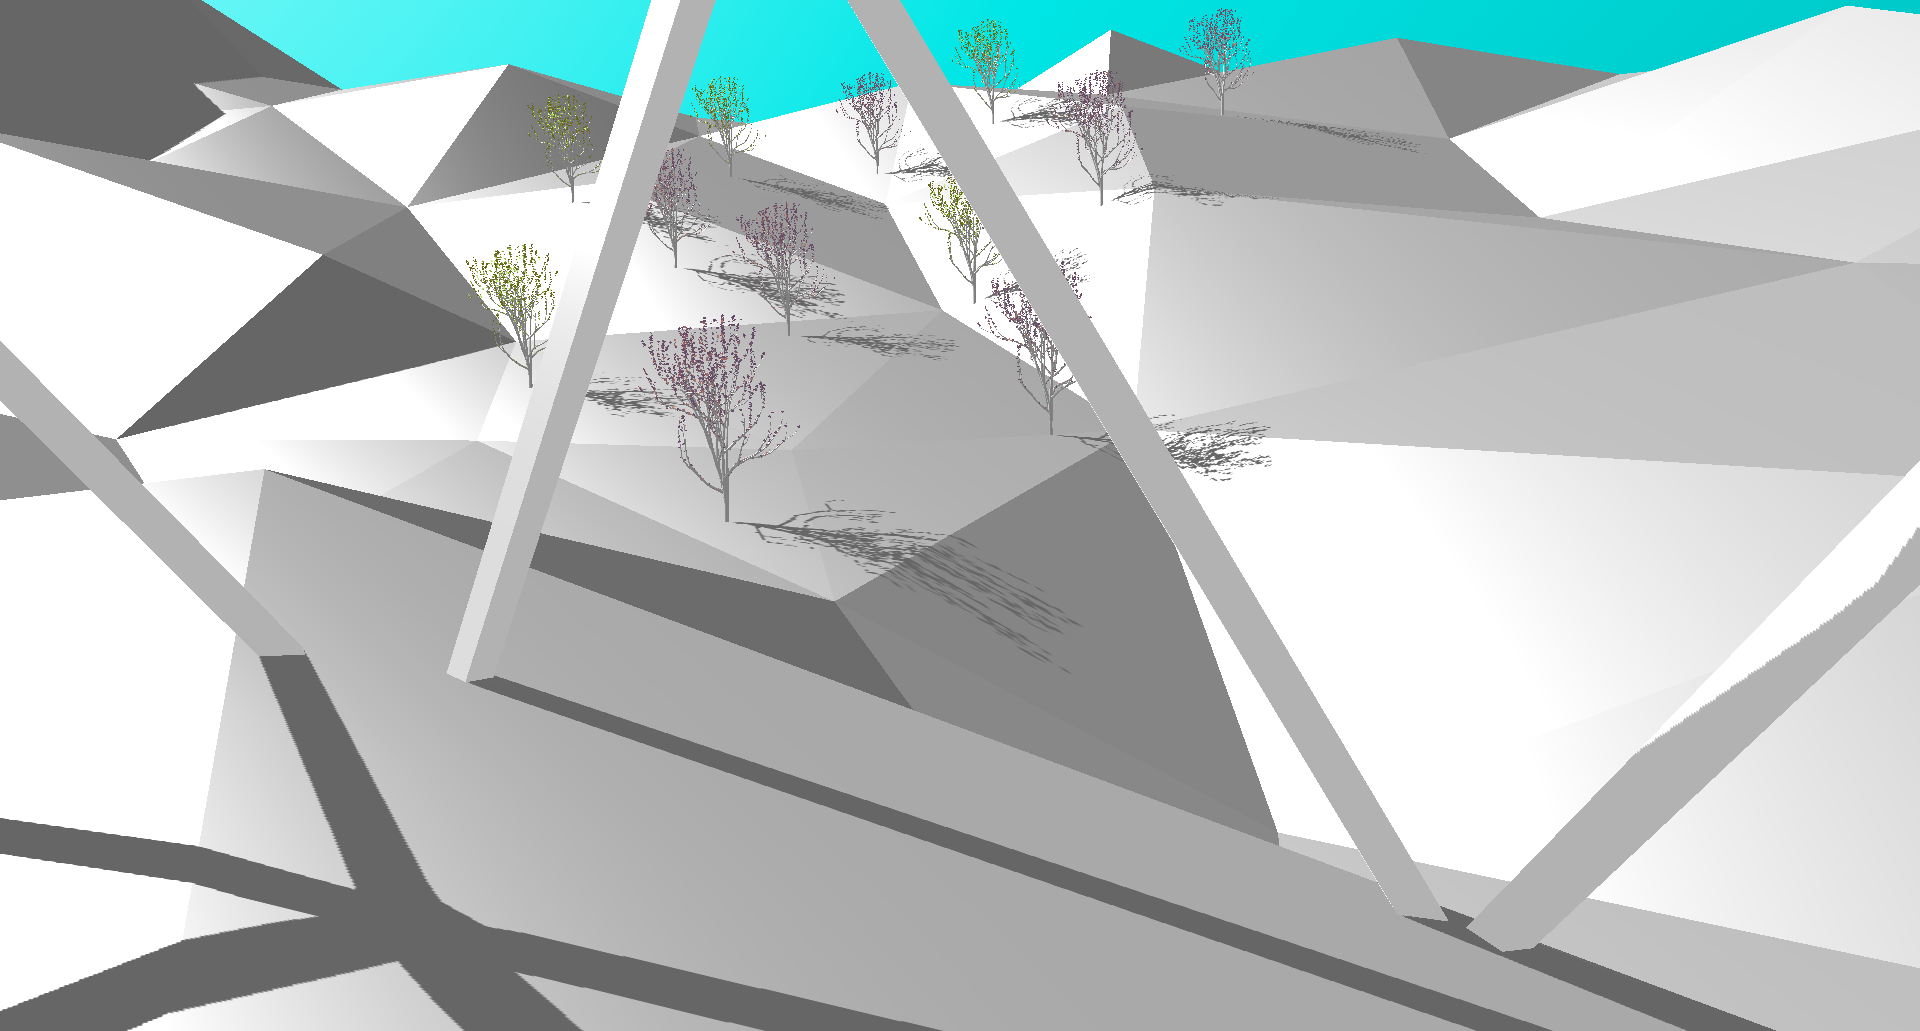
\includegraphics[width=5.5cm]{sdsm_assets/sdsm_scene.png}
		\label{ref:sdsm_scene}
	}
	\caption{Eine Szene die weit entfernte und sehr nahe Schatten enthält.}
\end{figure}

%  SDSM Light View
\begin{figure}
	\centering
	\subfloat[PSSM] {
		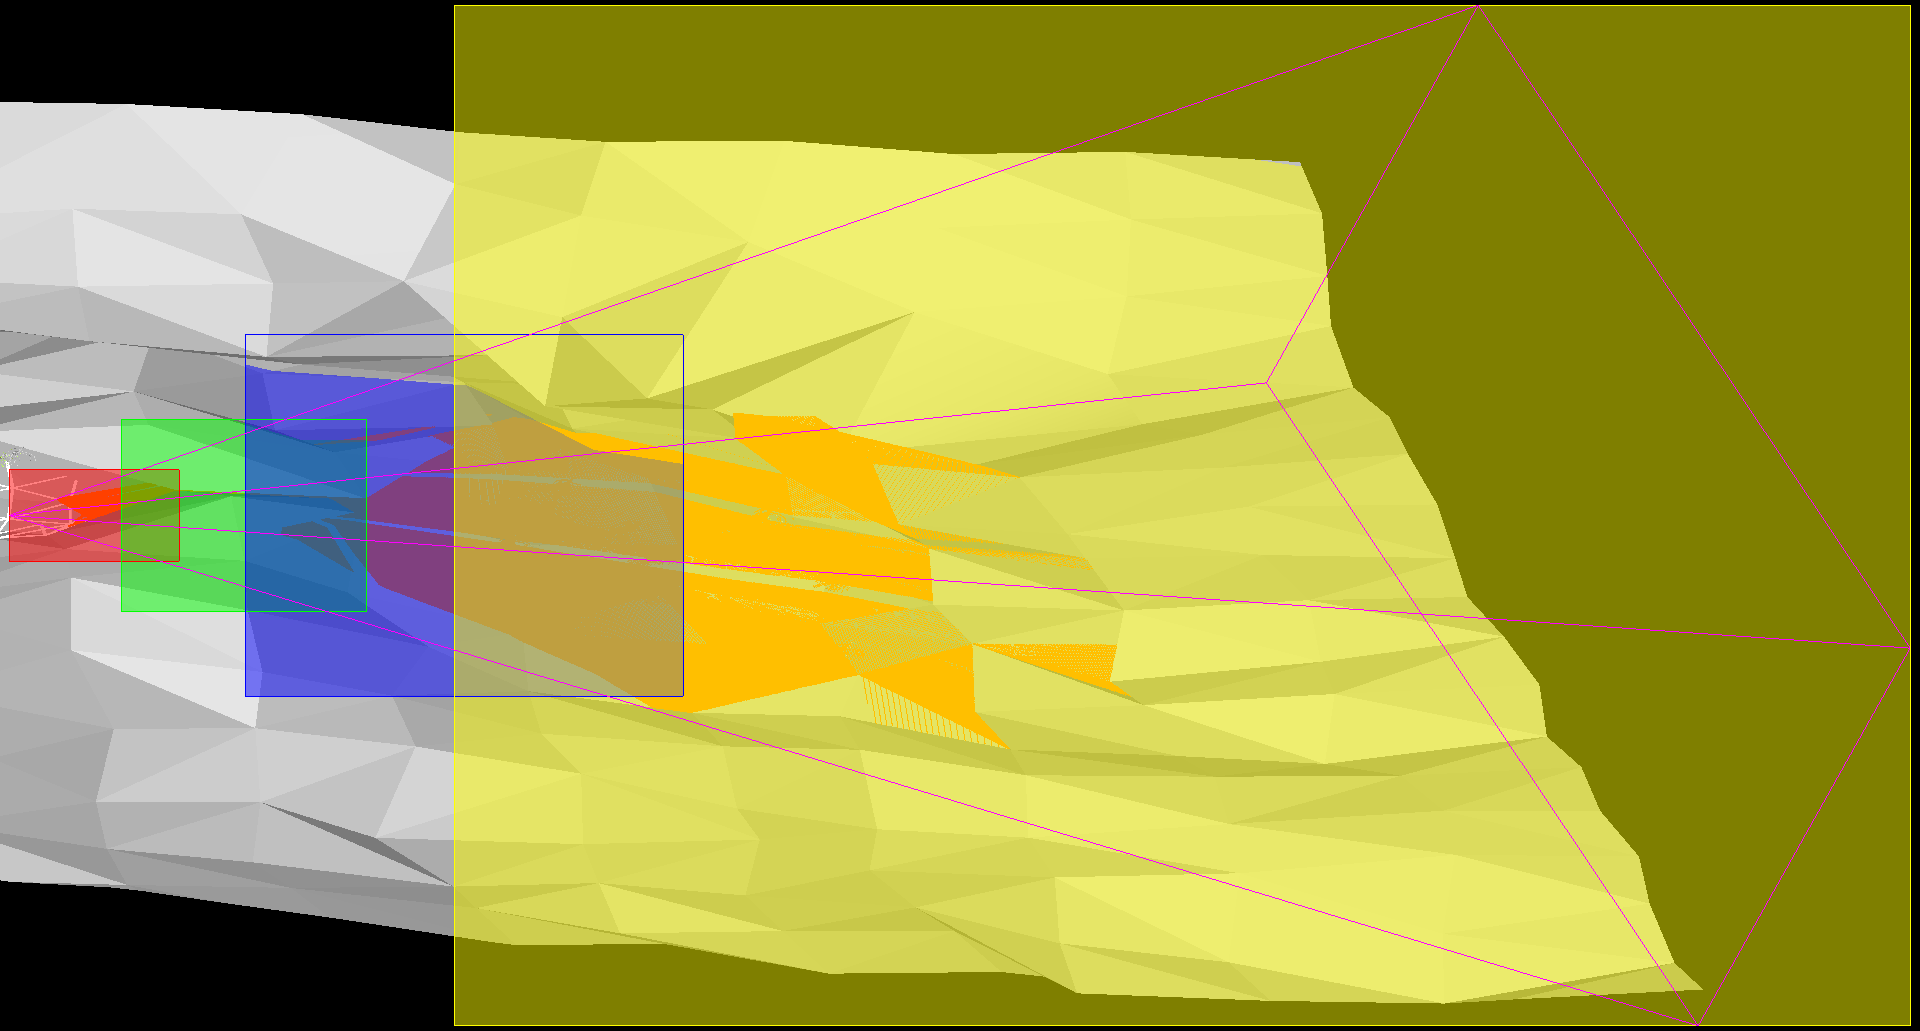
\includegraphics[width=5.5cm]{sdsm_assets/pssm_light_view.png}
		\label{ref:pssm_light}
	}
	\subfloat[SDSM] {
		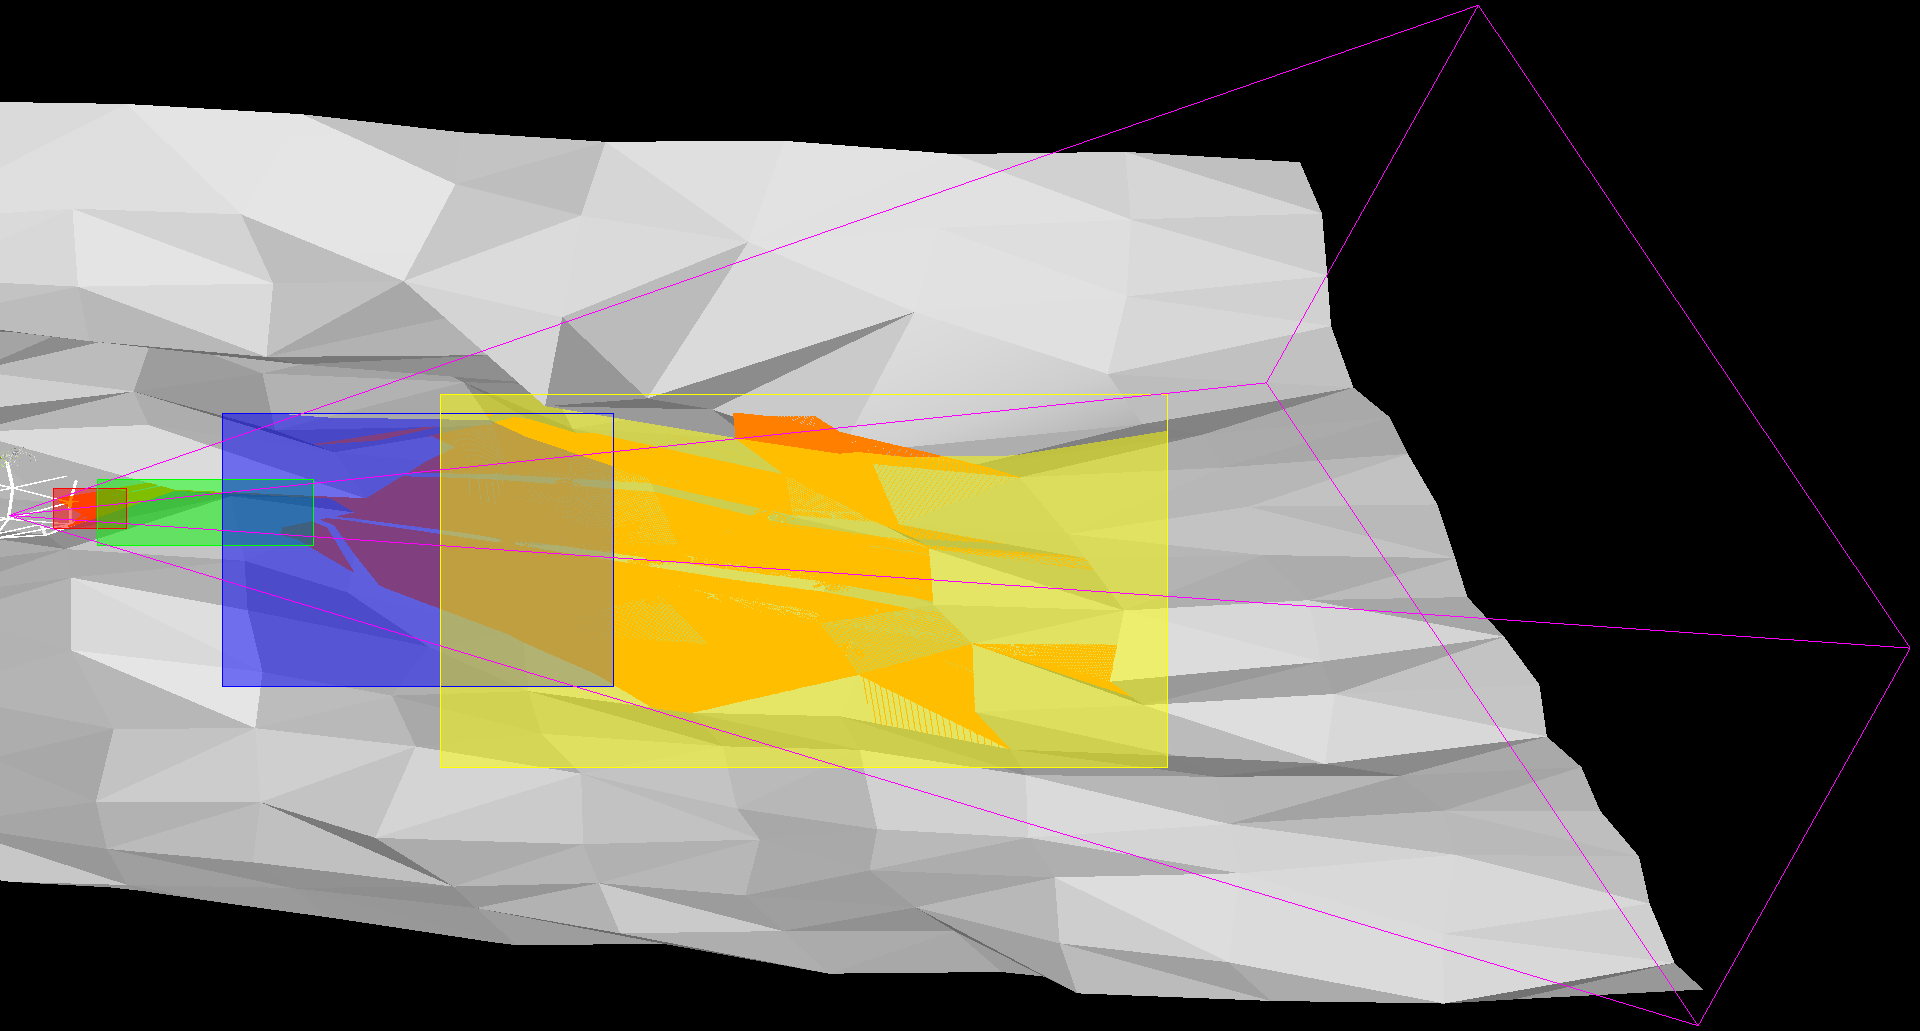
\includegraphics[width=5.5cm]{sdsm_assets/sdsm_light_view.png}
		\label{ref:sdsm_light}
	}

	\caption{Visulaisierung der von den Shadow Maps abgedeckten Bereichen mit PSSM und SDSM aus der Sicht des Lichtes.}
\end{figure}



% SDSM
\subsection{Implementierung}

% Rendern der Shadow Map
Die Shadow Maps für die Kaskaden werden mittels Texture Arrays realisiert, wobei jede Kaskade einen eigenen Layer in dem Array erhält.
Beim Rendern der Shadow Map transformiert der Vertex Shader die Geometrie zunächst nur in den World Space und nicht direkt in das Frustum der Shadow Map.
Der Geometry Shader klont dann die Geometrie und transformiert sie für jede Kaskade mit der dazugehörigen Projektionsmatrix in das Shadow Map Frustum um sie in den entsprechenden Layer der Shadow Map zu rendern.
Anstatt die Near Plane des Shadow Map Frustums zu verschieben, um Geometrie die aus der Sicht des Lichtes vor dem Camera Frustum liegt zu berücksichtigen, wird an der Near Plane des Shadow Map Frustums der Tiefenwert geclampt.

% Temporäre Licht Projektion
Um die Bounding Boxen der Geometrie in den einzelnen Kaskaden zu berechnen, müssen die Koordinaten im Light Space auf den Bereich $[0, 1]$ gemappt werden.
Hierzu werden die Eckpunkte im Screen Space in die Welt, und anschließend in den Light Space transformiert, wo dann deren Axis Aligned Bounding Box auf $[0, 1]^3$ projiziert wird.
So ist es garantiert, dass die Koordinaten sämmtlicher sichtbarer Geometrie im Light Space ohne clamping in einer Textur gespeichert werden können.

% Reduktion 1 & 2
Die beiden Reduktionen werden jeweils in einem Compute Shader ausgeführt.
Jeder Thread liest 1 bis 4 Einträge pro zu reduzierendem Wert ein.
Jede Thread Gruppe (von 256 Threads) generiert einen neuen Eintrag pro Wert.
Ausserdem versuchen wir die Zugriffsmuster auf den Shared Memory so weit es geht zu optimieren und Bank Conflicts zu vermeiden \cite{reduction}.
Um so mehr verschiedene Werte auf einmal reduziert werden, desto mehr können idle Zeiten von Threads in den Thread Gruppen vermieden werden.

Anstatt nach einer halbierung der Daten die eine Hälfte der Threads ihre Arbeit beendigen zu lassen, wird der erste zu reduzierende Wert von der ersten Hälfte der Threads, und die zweite zu reduzierende Wert von der zweiten Hälfte der Threads weiter bearbeitet und so weiter, bis jeder Thread sich nur noch um höchstens einen Wert kümmern muss.
Damit die Arbeit so aufgeteilt werden kann, müssen alle Reduktionsprobleme vom selben Typ sein.
\begin{equation}
  far = \max\{ depth \} = 1 - \min \{ 1 - depth \}
\end{equation}
Maximierungsprobleme werden während der Reduktionen Minimierungsprobleme betrachtet.
Durch die Addition von $1$ verlässt der zu reduzierende Wert den Wertebereich $[0, 1]$ nicht.
Dies gilt analog für die Max-Corners der Bounding Boxen.

Die Reduktionsergebnisse werden in 1D Texturen gespeichert.
So wird die Anzahl der Threads, die in einem Reduktionsschritt keine sinnvollen Daten einlesen, minimiert.

% In der zweiten Reduktion werden insgesammt $| \{min, max\} \times \{X, Y, Z\} \times \{0, 1, 2, 3\} | = 24$ Werte berechnet.
% Um die Vektorarithmetik der GPU auszunutzen empfiehlt es sich jeweils die vier Kaskaden in einen Vektor zusammen zu fassen, so dass noch 6 Vektoren reduziert werden, die jeweils in einer 4 Kanal Textur gespeichert werden.



% Keks
TODO irgendwas vergessen?


% SDSM
\subsubsection{Erster Versuch}
Im ersten Ansatz haben wir die Reduktionen für die tatsächliche Near und Far Distanz sowie die Bounding Boxen der Geometrie in den Kaskaden auf der GPU berechnet.
Das Ergebnis haben wir auf die CPU zurück gelesen um aus den Near und Far Distanzen die Partition zu berechnen, bzw. aus den Bounding Boxen das Frustum für die entsprechende Shadow Map.
Um zu vermeiden, dass der CPU auf die GPU warten muss, haben wir die Ergebnisse aus dem vorherigen Frame, bzw. von vor zwei Frames genutzt, da deren Berechnung dann schon abgeschlossen sein sollte.
Um Bewegungen der Kamera zu kompensieren, haben wir die Ergebnisse aus dem Camera Space des vergangenen Frames in die Welt transformiert und von dort in den aktuelle Camera Space.
Was wir nicht kompensieren konnten, war das erscheinen neuer Geometrie, die durch die Bewegung der Kamera sichtbar wurde.
Das hat z.B. zu Bereichen zwischen den Kaskaden geführt, die nicht von einer Shadow Map abgedeckt wurden.
Selbst wenn wir zur Sicherheit einen Rand in die Shadow Map einbauen, was nicht im Sinne von SDSM ist, können schnelle Bewegungen nicht kompensiert werden.

% SDSM
\subsubsection{Zweiter Versuch}
Dieses Problem haben wir gelöst, indem wir am Anfang jedes Frames einen Depth Only Pass gerendert haben.
Anschließend haben wir darauf die Near und Far Distanz wie zu vor berechnet.
Anstatt diese auf die CPU zurück zu lesen, haben wir die Partition in einem Compute Shader auf der GPU berechnet.
Nachdem die Bounding Boxen der Kaskaden berechnet waren, haben wir daraus ebenfalls auf der GPU die Projektionsmatrizen für die Shadow Maps berechnet.


% SDSM
\subsubsection{Sheared Sample Distribution Shadow Maps}
Wenn das Licht schräg (geneigt) von der Seite einfällt, sind die Shadow Map Frusta entlang ihrer Z-Achse oft sehr ausgedehnt.
% Auf der Licht zugewandten Seite des Frustums liegen abgetastet Punkte einer bestimmten Höhe oft näher am Licht, als die Punkte auf der Licht abgewandten Seite.
Dadurch wird die Genauigkeit bei der Quantifizierung der Tiefe in der Shadow Map verschlechtert.

%\begin{figure}
%	\centering
%	\begin{tikzpicture}[x=1cm,y=1cm] 
		
%		\draw [] (-1.5, -1) rectangle (1.5, 1);
%		\draw [] (-1.5*0.8, -1*0.8) rectangle (1.5*0.8, 1*0.8);
%		\draw [] (-1.5, -1) -- (-1.5*0.8, -1*0.8);
%		\draw [] ( 1.5, -1) -- ( 1.5*0.8, -1*0.8);
%		\draw [] ( 1.5,  1) -- ( 1.5*0.8,  1*0.8);
%		\draw [] (-1.5,  1) -- (-1.5*0.8,  1*0.8);

%		\draw [rotate around={45:(0,0)}] ({-sqrt(1.5^2 + 1^2)},{-sqrt(1.5^2 + 1^2)}) rectangle ({sqrt(1.5^2 + 1^2)}, {sqrt(1.5^2 + 1^2)});
		
		% Light Ray
%		\draw [->] (-3, 3) -- (-2, 2);
%		\draw [->] (-3.5, 2.5) -- (-2.5, 1.5);
%		\draw [->] (-2.5, 3.5) -- (-1.5, 2.5);
		
%		\draw (1,1) -- (1,4) -- (5,4) -- (5,1) -- (1,1);
		
%		\draw [dotted, thick] (1,4) -- (1,5) node [above] {$x_1$};
%		\draw [dotted, thick] (5,4) -- (5,5) node [above] {$x_2$};
		
%		\draw [dotted, thick] (5,1) -- (6,1) node [right] {$y_2$};
%		\draw [dotted, thick] (5,4) -- (6,4) node [right] {$y_1$};
	
%	\end{tikzpicture}
%\end{figure}

%  SDSM Shear
\begin{figure}
	\centering
	\subfloat [Sample Distribution Shadow Maps] {
		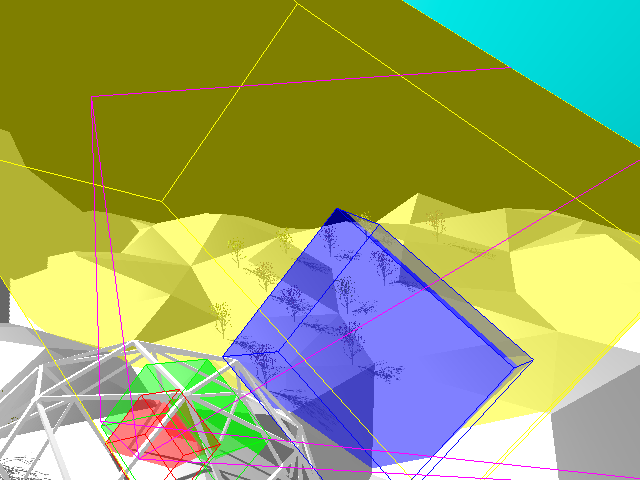
\includegraphics[width=5.5cm]{sdsm_assets/sdsm_no_shear_volumes_small.png}
		\label{ref:sdsm_light}
	}
	\subfloat [Sheared Sample Distribution Shadow Maps] {
		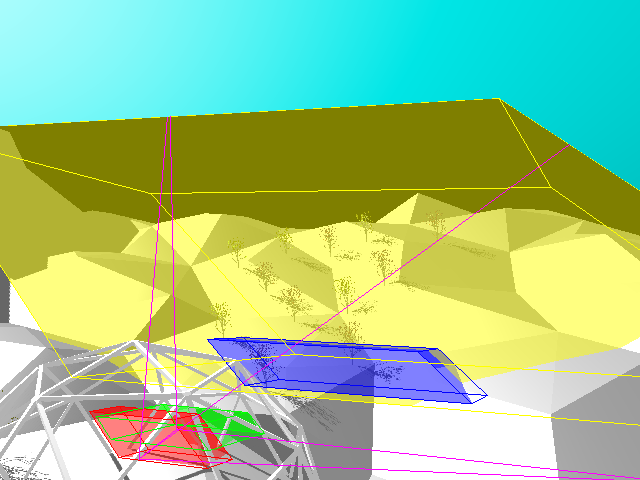
\includegraphics[width=5.5cm]{sdsm_assets/sdsm_shear_volumes_small.png}
		\label{ref:sdsm_light}
	}
	
	\caption{Visualisierung der Shadow Map Frusta.}
\end{figure}

Unsere Lösung für dieses Problem ist eine einfache Scherung des Light Spaces.
Die X-Achse des Camera Spaces wird im Light Space auf die Y-Achse abgebildet.
So haben Koordinaten, die im Camera Space die gleiche Höhe (Y-Achse) haben, im Light Space die gleiche Tiefe (Z-Achse).

Auch wenn wir es so geschafft haben in vielen Situationen die Shadow Map Frusta weiter zu verkleinern, ist durch die Scherung die Filterbarkeit der Momente \cite{msm} nicht mehr gegeben.
Es war relativ einfach Situationen zu provozieren, in denen die Scherung keine Sinnvolle transformation erzeugt hat.

TODO soll das hier auch mit rein?



% Main
\section{Volumetric Obscurance}

Volumentric Obscurance wird aus dem Screenspace berechnet. Allgemein wird für jeden Punkt der Szene, der auf
dem Bildschirm gezeichnet wird, eine gegebene Umgebung (z.B. eine Einheitskugel um diesen Punkt) betrachtet.
Für diese Umgebung wird der Anteil an Geometrie berechnet, die für den Beobachter sichtbar ist. Je mehr Geometrie
verdeckt ist, umso mehr wird der korrespondierende Pixel abgedunkelt um so den ausbleibenden Lichteinfall,
also den Schatten, zu simulieren.
Das entsprechnde mathematische Modell sieht wie folgt aus \cite{voPaper}
$$
V(P) = \int_{X} \rho (d(P,x))O(x)dx
$$
Dabei ist $X$ die Nachbarschaft um den Punkt $P$, $O$ ist die Verdeckungs-Funktion. Diese
ist 0, falls Verdeckung stattfindet, sonst 1. $\rho$ ist eine abfallende Funktion
die 1 bei P ist und mit der Distanz abfällt. Wie in \cite{voPaper} beschrieben, ist der 
sichtbare Effekt jedoch nur sehr minimal, weshalb diese Funktion als konstant angesehen 
wird \cite{voPaper}

\subsection{Line Sampling}
Line Sampled Volumetric Obscurance nutzt (möglichst) zufallsverteilte Samples innerhalb auf der auf den
Screenspace projezierten Umgebung des Punktes. In der hier implementierten Version (die ebenfalls in
\cite{voPaper} beschrieben wird) wird die Einheitskugel um den Punkt P in der Szene betrachtet.
Sei nun $d$ die Tiefe des Punktes $P$. Dann ist die allgemeine Verdeckungsfunktion für eine andere Tiefe
$z$ :
$$
f(z) = \begin{cases} 1 &  \text{für } z \leq d \\ 0 & \text{für } z > d \end{cases}
$$
Für die hier vorgestellte Implementierung wird eine feste Anzahl $N$ an Samples verwendet.
Dann ergibt sich daraus:
$$
F_{N}(z_0, \dots, z_N) = \sum_i^N \frac{v_i}{2 \cdot z_{s_i}} \max{(\min{(z_{s_i}, d_{r_i})} + z_{s_i}, 0)}
$$
Dabei ist $z_i$ die Tiefe des i-ten Samples im Depth-Buffer, $d_{r_i}$ ist die Tiefe $z_i$ gemapped in die
betrachtete Umgebung des Punktes $P$, $z_{s_i} = \sqrt{1 - x_i^2 - y_i^2}$. $(x_i, y_i)$ ist die Position des
i-ten Samples auf der Einheitsscheibe (also der Querschnitt der Einheitskugel, die den Punkt P 
beinhaltet und dessen normale parallel zur Blickrichtung liegt). \newline

\begin{figure}
	\centering

	\input{LineSamples.pdf_tex}
	\label{ref:lineSample}

	\caption{Line Sampling}
\end{figure}

\subsubsection{Implementierung}
	\textbf{Line Sampling Pseudo Code}\\
	\begin{algorithm}[H]
		
		\Fn{LineSampling(nSamples, depth)}{
			sumSamples = 0\;
			sumVolume = 0\;
		    \For{i = 0 $\rightarrow$ nSamples - 1}{
		    	radius = rand()\;
		    	$\alpha$ = rand()$\cdot 2\pi$\;
		    	weight = $\sqrt{1 - radius^2}$\;
		    	p = $(\cos{(\alpha)} \cdot radius,\sin{(\alpha)} \cdot radius)^T$\;
		    	sumSamples = sumSamples + weight $\cdot$ SamplePoint(p, depth)\;
		    	sumVolume = sumVolume + weight\;
		    }
		    return $\frac{sumSamples}{sumVolume}$ \;
		}
		
		\Fn{SamplePoint(p, depth)}{
			\textit{hier wird ein einzelner Punkt gesampled, wie oben beschrieben [TODO?]}
		}
		
		\Fn{rand()}{
			return \textit{zufälliger Wert im Intervall [0,1]}\;
		}
		
	\end{algorithm}

\subsubsection{Ergebnisse}
TODO

\subsection{Area Sampling}
Line Sampling Volumetric Obscurance nutzt zufallsverteilte Samples um die Verdeckung einer
Raumregion zu approximieren. Ein alternativer Ansatz ist Area Sampling. Anstatt zufallsverteilter Samples
versucht Area Sampling die Verteilung über das Mittel statistischer Größen zu ermitteln. Dafür
wird der selbe Ansatz wie bei Variance Shadow Maps \cite{vsmPaper} verwendet. Beim Line Sampling
nutzten wir samples auf dem DepthBuffer, beim Area Sampling schreiben wir stattdessen die ersten beiden
Momente $(z^1, z^2)$ für jeden Pixel im Screenspace heraus und filtern diese Größe über einen Bereich, der
Abhängig von der Tiefe ist (analog zu der von der Tiefe abhängigen, auf den Screenspace projezierten Umgebung
im Abschnitt Line Sampling). In unserer Implementierung bestimmen wir in einem Renderschritt [blödes Wort]
die Tiefe der Szene $(z)$ aus Sicht der Kamera und schreiben das Tupel $(z, z^2)$ in den ersten beiden
Farbkanälen einer Textur. Bevor wir die finale Szene rendern mipmappen wir die Textur.
In der Nachbearbeitung (Compose Schritt) der gerenderten Szene greifen wir abhängig von der Tiefe an jedem
Pixel auf die entsprechende Mipmap-Ebene zu, welche die so gefilterten Momente enthält.
Über das abgegriffene Tupel $t = (z_f, z_f^2)$ bekommen wir dann einen Approximierten Mittelwert 
$\mu = t[0]$ und die gemittelte Varianz $\sigma^2 = t[1] - t[0]^2$. Dann lässt sich der Verdeckungsfaktor 
folgendermaßen abschätzen:
$$
V_c(z_0, z_1, a, b) = a\cdot(z_1^2 - z_0^2) / 2 + b \cdot (z_1 - z_0)
$$
wobei $z_0$ und $z_1$ die Start- und Endtiefe der Umgebung des betrachteten Punktes P sind und die 
Koeffizienten $a$ und $b$ definiert sind als:
$$
a = \frac{-1}{2 \cdot \sigma}; \quad b = -a \cdot (\mu + \sigma)
$$

\subsubsection{} \textbf{Pseudocode für Area Sampling:} \\
\begin{algorithm}[H]
    \Fn{AreaSampling(momentsMipmap, uv)}{
		unfilteredMoments = getMomentsFromLevel(momentsMipmap, uv, 0)\;
		depth = unfilteredMoments[0]\;
		r = getRadiusInScreenspace(depth)\;
		mipMapLevel = $\log_2 (\frac{1}{1 - r})$ \;
		moments = getMomentsFromLevel(momentsMipmap, uv, mipMapLevel)\;
		$\mu$ = moments[0]\;
		$\sigma$ = $\sqrt{ \text{moments[1]} - \mu^2}$\;
		$a$ = $\frac{-1}{2 \cdot \sigma}$\;
		$b$ = $-a \cdot (\mu + \sigma)$\;
		$z_0$ = depth - r\;
		$z_1$ = depth + r\;
		vCoeff = $V_c(z_0, z_1, a, b)$\;
		return vCoeff\;
	}
\end{algorithm}
Dabei ist \textit{getMomentsFromLevel(mipmap, uv, level)} die Funktion, die von der Mipmap \textit{mipmap}
an der Stelle \textit{uv} den Texel an gegebenem \textit{level} abgreift. 

% Main
\section{Moment Shadow Mapping}

Um eine möglichst hohe Qualität an Schatten zu erreichen bieten sich verschiedene Verfahren an. Deswegen ist es wünschenswert für uns eine filterbare Shadow Map zu nutzen. Percentage Close Filtering eliminiert Aliasing Effekt durch samplen der Schadow Map und durch einen Filter Kernel.\cite{msm} 
Allerdings kann dies nur für einzelne Fragmente geschehen, da das Verfahren tiefenabhängig beim Schattentest ist.\cite{msm}
Es bietet sich daher an mit Momenten zu arbeiten. Variance Shadow Maps nutzen zwei Momente und bietet deshalb zusätzlich die quadrierte Tiefeninformation um die Shadow Map. Diese wird genutzt um PCF weiter zu approximieren und filterbare Shadow Maps zu nutzen.\cite{donnelly2006variance}
Wir werden das Hamburger Moment Shadow Mapping nutzen, welches 4 Momente generiert und den Variance Shadow Maps ähnlich ist. Zum filtern nutzen wir MSAA und zum einen Gauss Filter. Die Implementierung war denkbar einfach, da wir bereits DirectX Shader Code hatten, durch die Präsentation des Moment Shadow Mapping Papers\cite{msm}. Diesen haben wir für OpenGL umgesetzt.

% MSM
\subsection{Algorithmus}

Wir nutzen den Algorithmus Hamburger Moment Shadow Mapping. Dieser versucht das General Moment Problem zu lösen und stellt eine Verbesserung des VSM bzw. PCF dar. Hierfür nutzen wir Algorithmus 3 aus dem Moment Shadow Mapping Paper.\cite{msm} Der grundlegende Aufbau des MSM, ist dem der VSM sehr ähnlich, denn VSM ist hinsichtlich des MSM ein Spezialfall für 2 Momente. Für uns wünschenswert, ist aber eine Methode mit 4 Momenten.
Wir möchten eine möglichst scharfe untere Schranke nutzen, damit wir die Schattenwerte nicht überschätzen.\cite{msm}. 
Auch VSM löst dieses und der Vorteil liegt in der Vermeidung von Artefakten, wie etwa Surface acne. Übrig bleiben noch Artefakte wie Light Bleeding durch falsche Schattenintensitä. Da wir bisher eine untere Schranke haben überschätzen wird niemals die Werte niemals für die Schattenintensität. Allerdings können nocht Fehler wie etwa Light Bleeding auftreten. 
Eine weitere Vereinfachung in Richtung Hamburger MSM wird im Paper durchdurch Algorithmus 2 erreicht.
Algorithmus 2 bietet aber noch nicht die nötige Robustheit für eine Echtzeitanwendung.\cite{msm}
Letztendlich führt uns dies zu Algorithmus 3, welchen wir auch genutzt haben bzw. als Shader Code gegeben hatten. Dieser ist ein Spezialfall des Algorithmus 2 und liefert und  die gewünschte Schattenintensität. 
Light Bleeding und Aliasing werden vermindert und wir erhalten eine Schattenintensität, die sowohl helle als auch dunkle Werte gut einschätzen kann. Dies übertrifft die Ergebnisse von VSM und PCF bzw. erweitert und übertrifft die Ergebnisse umd Artefakte weiter zu verhinden. Dadurch erhalten wir qualitativ hochwertige Schatten ohne viel Leistung einzubüßen. Ausserdem ist dieser Algorithmus robust genug für Echtzeitanwendung, was in der Implementierung aufgezeigt wird. 
Da Algorithmus 3 auf double precision Werten aufbaut, welche zu Speicherintensiv wären, nutzt die Implementierung einen einfach Bias Moment Vector und im Paper wird gezeigt, dass dies nur zu kleinere Ungenauigkeiten führt.\cite{msm} Auch diesen Bias haben wir in unserer Implementierung genutzt. Wir hatten bereits Shader Code für DirectX vorliegen, da dieser bereits implementiert wurde. Diesen haben wir im weiteren Verlauf für OpenGL umgesetzt.

\subsection{Moment Based Volumetric Obscurance}
Für die Moment Based Volumetric Obscurance benötigen wir noch Gewichte aus dem Moment Shadow Mapping. Diese finden sich in Algorithmus 2 und werden in unserer Implementierung weiter genutzt.
Hierfür nutzen wir die Funktion $Es(f) = \sum w_i*f(z_i)$ \cite{mbvo} auf Basis von $S = \sum w_i*\delta$ aus dem MSM Algorithmus. Durch angleichen unserer Implementierung um die Gewichte $w_i$ zu erhalten, können wir die Funktion für das MBVO berechnen. Diese liefert uns den gewünschten Term für die Moment Based Volumetric Obscurance. Allerdings haben wir während der Implementierung noch kein stimmiges Bild erhalten, welches aber im Abschnitt der Implementierung weiter erläutert wird. Weiterführen wird der Algorithmus im Anhang erläutert, durch zusätzliche Notizen, welche wir für die Projekgruppe erhalten haben. Diese beziehen sich im speziellen auf die MBVO im Zusammenhang mit dem MSM.\cite{mbvo}

% MSM
\subsection{Implementierung}

Wir implementieren die Hamburger Moment Shadow Mapping Technik. 
Zuerst wird eine Moment Shadow Map gerendert. Der Unterschied zur normalen Shadow Map ist, das zusätzlich noch 4 Momente, bestehend aus der Tiefe der Shadow Map gespeichert werden. Diese reduntanten Tiefeninformationen können noch gefiltert werden. Wir verwenden hierfür einen Gauss Filter oder alternativ noch MSAA. Eine weitere Möglichkeit wäre Mip-Mapping. Da wir bereits eine Shadow Map rendern, müssen wir nur noch eine Funktion nutzen um die Momente zu generieren.
Im zweiten Schritt der Implementierung, wird ein gefiltertes Sample aus der Moment Shadow Map, sowie die Tiefe eines Shadow Map Fragments genutzt, um eine gefilterte Schatten Intensität zu erhalten.
Wir nutzen hierfür eine weitere Funktion um diese Berechnungen durzuführen und einen Wert für die Schattenintensität zu generieren, welchen wir im Programm nutzen können. Dies ist im Abschnitt Algorithmus bereits näher erläutert.
Im Shader haben wir dann folgendes angewendet um oben genanntes umzusetzen.
Das erstellen der Momente passiert in einem eignen Shader. Hierfür nutzen wir die Tiefe und speichern uns zusätzlich noch die Tiefe hoch 2, 3 und 4. Diese werden gesampelt und dann weiter an den Fragment Shader gereicht.
Im Fragment Shader, verarbeiten wir die Momente. Das heißt wir benutzen zwei Funktion um oben genannte gefilterte Samples zu generieren und diese dann in einer in eine Schattenintensität umzuwandeln. Hierfür haben wir den gegeben Direct X Shader in OpenGL übersetzt. Beachtenswert war, das Matrixtransformationen etwas anders gehandhabt werden als in DirectX und ein paar Standardfunktionen selbstgeschrieben werden müssen, was in den ersten Versuchen zu Fehlern in den Momenten geführt hat.

\begin{lstlisting}
void main()
{
    ivec3 pos = ivec3(gl_GlobalInvocationID.xyz);

    vec4 moments = vec4(0, 0, 0, 0);
    for (int i = 0; i < sampleCount; i++)
    {
        float depth = texelFetch(depthSampler, pos, i).x;
        float square = depth * depth;
        moments += vec4(depth, square, square*depth, square*square);
    }
    moments /= sampleCount;

	vec4 fragMoments = transpose(mat4(	
	-2.07224649,32.23703778,-68.571074599,39.3703274134,
    13.7948857237,-59.4683975703,82.0359750338,-35.364903257,
    0.105877704,-1.9077466311,9.3496555107,-6.6543490743,
    9.7924062118,-33.7652110555,47.9456096605,-23.9728048165))
	* moments;
	fragMoments.x += 0.035955884801;

    imageStore(momentImage, pos, fragMoments);
}
\end{lstlisting}

Hier wird im create\_moments\_Shader die Momente
$$
z, z^2, z^3, z^4
$$
$z$ entpricht der Tiefe aus dem Depth Buffer.
generiert und durch eine Matrix transformiert damit eine 16-bit Quantifikation ausreicht.

\begin{lstlisting}
void sampleOptimized4MomentsShadowMap(out vec4 out4Moments, 
	vec4 shadowMapValue)
{
    shadowMapValue.x -= 0.035955884801f;
    out4Moments = transpose(mat4(     			
    	0.2227744146,0.0771972861,0.7926986636,0.0319417555,
    0.1549679261,0.1394629426,0.7963415838,-0.172282317,
    0.1451988946,0.2120202157,0.7258694464,-0.2758014811,
    0.163127443,0.2591432266,0.6539092497,-0.3376131734))
    * shadowMapValue;

}
\end{lstlisting}
Hier werden die Sample rückgerechnet, damit diese besser in eine Textur schreiben können.
Dies geschieht im Fragment\_Shader
\begin{lstlisting}
float computeMSMShadwowIntensity(vec4 in4Moments, float depth, 
	float depthBias, float momentBias)
{
    vec4 b = mix(in4Moments, vec4(0.5,0.5,0.5,0.5), momentBias);
    vec3 z;
    z.x = depth-depthBias;
    float L32D22= -b.x * b.y + b.z;
    float D22= -b.x * b.x + b.y;
    float SquaredDepthVariance=-b.y * b.y + b.w;
    float D33D22=dot(vec2(SquaredDepthVariance,-L32D22),
                     vec2(D22,                  L32D22));
    float InvD22=1.0/D22;
    float L32=L32D22*InvD22;
    vec3 c=vec3(1.0,z.x,z.x*z.x);
    c.y-=b.x;
    c.z-=b.y+L32*c.y;
    c.y*=InvD22;
    c.z*=D22/D33D22;
    c.y-=L32*c.z;
    c.x-=dot(c.yz,b.xy);
    float p=c.y/c.z;
    float q=c.x/c.z;
    float r=sqrt((p*p*0.25)-q);
    z.y=-p*0.5-r;
    z.z=-p*0.5+r;
    vec4 Switch=
        (z.z<z.x)?vec4(z.y,z.x,1.0,1.0):(
        (z.y<z.x)?vec4(z.x,z.y,0.0,1.0):
        vec4(0.0,0.0,0.0,0.0));
    float Quotient=(Switch.x*z.z-b.x*(Switch.x+z.z)+b.y)
                  /((z.z-Switch.y)*(z.x-z.y));
    return 1-clamp(Switch.z+Switch.w*Quotient,0,1);
    
}
\end{lstlisting}
\begin{lstlisting}
float simpleShadowTerm()
{
    
    int index = getCascade();

    vec4 lightViewPosition=cascadeViewMatrix[index]*vec4(worldPosition, 1.);
    vec2 uv=vec2(lightViewPosition.xy*0.5+0.5);
    vec4 shadowMapValue=texture2DArray(shadowMapSampler, vec3(uv,index));
    float depth=lightViewPosition.z*0.5+0.5;
    vec4 shadowMapMoments;
    sampleOptimized4MomentsShadowMap(shadowMapMoments,shadowMapValue);
    return computeMSMShadwowIntensity(shadowMapMoments,depth,0.005,3e-5);
\end{lstlisting}
Letzendlich können wir die Schattenintensität berechnen, auf Basis des Algorithmus 3 aus dem MSM Paper.\cite{msm}
Die Funktionen rufen wir in der simpleShadowTerm() Funktion auf und geben diese letzendlich als Wert für die Textur zurück.

\subsection{Moment Based Volumetric Obscurance}
Für das Moment Based Volumetric Obscurance benutzen wir die gleiche Herangehensweise. Allerdings hat es sich herausgestellt, dass die Transformation für 4 Momente zu Artefakten führt. Dies entspricht dem samplen im Fragment Shader aus der Implementierung des Moment Shadow Mapping. Deswegen wurde dieser Schritt für das Moment Based Volumetric Obscurance entfernt. Das samplen bei der Generierung der Momente bleibt erhalten. Problematisch ist hier die Varianz um einen möglichst korrekten Wert für die Vomuletric Obscurance zu erhalten. Möglicherweise sind hier noch weitere Feineinstellung und Variablen nötig um ein stimmiges Bild zu erhalten. Technisch gesehen, funktiert das Verfahren aber.
\begin{lstlisting}
// Modified MSMShadowIntensity function
void computeMSMWeights(out vec3 Weight, out vec3 outz, vec4 in4Moments, 
float depth, float depthBias, float momentBias)
{

vec4 b = mix(in4Moments, vec4(0.5,0.5,0.5,0.5), momentBias);
//
...
//
Weight.x=(z.y*z.z-b.x*(z.y+z.z)+b.y)/((z.x-z.y)*(z.x-z.z));
Weight.y=(z.x*z.z-b.x*(z.x+z.z)+b.x)/((z.z-z.y)*(z.x-z.y));
Weight.z=1.0-Weight.x-Weight.y;
}
\end{lstlisting}
Das ganze haben wir in einem Compose Shader implementiert und die Funktionen aus dem MSM weitestgehend übernommen.
Wir wählen ebenfalls 4 Momente um die Volumetric Obscurance zu approximieren und berechnen die benötigten Gewichte durch eine Abbänderung der MSM Funktionen. Dies ist ebenfalls im Abschnitt Algorithmus näher erläutert.
Im Shader wird die Funktion zum generieren der Schattenintensität um eine Berechnung der Gewichte erweitert, sodass diese für die Volumetric Obscurance nutzbar ausgegeben werden können. Im weiteren Verlauf wird dies noch mit dem Area Sampling aus der Volumetric Obscurance erweitert. Dies ist im Abschnitt Volumetric Obscurance näher erläutert.
Die MBVO färbt Konturen der Geometrie sehr dunkel ein und hat Ähnlichkeiten mit einem Cell Shading Effekt.



\section{Fazit}


% Fazit
\subsection{Sample Distribution Shadow Maps}
SDSMs sind sehr robust und benötigen keine möglicherweise von Hand zu optimierenden Parameter um gute Ergebnisse zu liefern.
PSSMs können oft ähnlich gute Ergebnisse liefern wenn sie optimal eingestellt sind.
Allerdings gilt dies meist nur für eine bestimmte Sicht auf die Szene.
Befindet sich mehr oder weniger Geometrie in unmittelbarer nähe zur Kamera, so liefert PSSM keine guten Ergebnisse mehr.
SDSM passt ihre Z-Partitionen adaptiv an die veränderte Sichtbarkeit an.
Dies ist möglich, da SDSMs die tatsächliche Near Plane kennen, wo PSSMs nur eine untere Schranke hierfür kennen, die sich aus der Camera Projektion ergibt.

% Verbesserung der MSM durch SDSM
% TODO erstmal nur skizziert!
SDSMs optimieren nicht nur die Ausnutzung der Shadow Map Auflösung, sondern auch die Ausnutzung der zur Verfügung stehenden Genauigkeit in der Shadow Map, da die Shadow Map Frusta in allen drei Dimensionen eng um die sichtbare Geometrie gelegt wird.
Dies kommt dem Moment Shadow Mapping zu gute, da so feinere Abstufungen in den Momenten erlaubt werden können.


% Fazit
\subsection{Moment Shadow Mapping}
Das Moment Shadow Mapping bietet uns Schatten mit hoher Qualität, welche auch sehr gut zur Geltung kommen. Artefakte wie Aliasing und Light Bleeding werden stärker gemindert als bei VSM möglich. Ausserdem funktiort die Implementierung sehr einfach. Das Verfahren ist schnell und bietet beim filtern viele Freiheiten. Wir nutzen Gauss und 1xMSAA-16xMSAA welches verschiedene Ergebnisse liefert.
Auch dies hat sich kaum auf die Performance ausgewirkt und wir sind mit dem Ergebniss sehr zufrieden.
Im direkten Verlgleich zu PCF fällt auf, das MSM weitere Artefakte unterbindet. Im Verlgleich zu VSM bieten die 4 statt 2 Momente ebenfalls einen Vorteil. Light Leeking wird effektiv vermindert, was bei VSM nicht der Fall ist.
Für die Zukunft wollen wir noch weiteres filtern testen, um das Aliasing weiter zu vermindern.


% Fazit
\subsection{Moment Based Volumetric Obscurance}
Das Verfahren zur Moment Based Volumetric Obscurance war ebenfalls leicht umzusetzen, da sich die Implementierung kaum vom MSM unterscheidet. Aufgrund von anfänglichen Artefakten, haben wir aber eine sample Methode entfernt, welches ein stimmigeres Bild ergab. Insgesamt ist das Bild aber noch nicht stimmig genug, hier müssen wir weiter mit den Werten experimentieren, damit keine Cell Shading Optik erscheint. Interessant ist das Moment Based Volumetric Obscurance aber ebenfalls für grossflächuiges Filtern, welches noch weitere Experimente benötigt.



% Literaturverzeichnis:
\bibliography{lit}
\bibliographystyle{alpha}

\end{document}

